% !TeX root = ../main.tex
\chapter{托卡马克非热化电子相关理论及诊断}\label{sec:chapt2}

%\section*{引言}
\vspace{1em}
如果说算法是程序的骨架,那么理论便是程序的灵魂。本章主要介绍动理学计算程序的理论基础。首先介绍均匀磁场背景中非热化电子在静电场下演化的基本物理过程 ,然后通过动理学方程定量描述不同物理过程对电子速度分布函数的影响,最后介绍与非热化电子相关的诊断。

\section{非热化电子相关理论研究}

非热化电子演化涉及到加热\cite{RN1454}、磁重联\cite{RN1917}、以及粒子输运\cite{RN1744}	等过
程,在托卡马克放电中占据着非常重要的地位。非热化电子的研究涉及到速度分布函数的演化 ,不满足
热分布的速度分布函数在碰撞、散射、电磁场扰动、耗散、不均匀背景磁场分布等条件下如何演化是人
们一直关心的问题,动理学方程是描述这类问题的主要手段。通过求解动理学方程可以定量分析电场、
磁场以及电磁波对速度分布的影响,因此动理学模型的选择尤为重要。本节首先定性分析非热化电子在
理想背景中的速度演化行为,然后分别介绍不同物理过程涉及的动理学方程。
\subsection{基本物理过程}
首先我们定性描述非热化电子演化过程中伴随的物理过程。为了参考托卡马克物理条件同时适当简
化物理模型,我们忽略磁场梯度,只局限于分析均匀背景磁场中温度为$T_e$的等离子体在平行磁
场方向电场驱动下的演化。如\autoref{fig:nts}	所示,首先电子会受到库伦碰撞和电场力的相互作
用。 根据卢瑟福散射模型,电子运动碰撞阻力和电子速度的平方成反比,电子运动速度越快,受到的阻
力越小。当电子受到电场的驱动力大于电子的碰撞阻力,电子将会不断受到加速。CONNOR给出了一个
临界电场$E_c=(n_e e^3 lnΛ)/(4πϵ_0^2 c^2 )$\cite{RN1875},当$E>E_c$时,对于速度大于临界速度$v_c^2=(n_e e^3 lnΛ)/(4πϵ_0^2 E)$的电子群,由于碰撞阻尼小于电场驱动力,这部分的电子将会受到
加速从电场中获得能量发展成逃逸电子\cite{RN1744},这种大于临界速度形成的逃逸电子称为初级逃逸
电子。获得足够能量的初级逃逸电子和背景电子有一定几率发生大角度碰撞,当碰撞后的两个电子速度均大
于逃逸临界速度,那么一个逃逸电子就有可能会通过大角度碰撞效应产生两个逃逸电子,然后二变四,四变
八,逃逸电子的数量将呈指数增长,这种现象叫雪崩逃逸\cite{RN1827}\cite{RN1793}。当碰撞后的电子
速度小于逃逸临界速度时,逃逸电子数量便会减少,退化为热电子。随着逃逸电子速度增加到十几兆电
子伏特,同步辐射阻尼机制开始变得重要,直到辐射阻尼和电场力达到平衡,这使得电子的能量存在最
高上限。同时,由于等离子体中存在各种模式的电磁波,当高能电子速度和波满足$ω=\vk∙\vv+nω_{ce}
(n∈Z)$时会通过共振效应将能量传递给波,波被激发后又会反过来和高能电子相互作用通过电磁湍动过
程使高能电子发生角度散射,导致高能电子平行方向动能散射到垂直方向形成超热电子(垂直方向平均能
量$\sim100keV$)。超热电子又会在电场驱动下加速,当速度再次满足共振条件时又会进入到下一个散
射循环,同时超热电子也可能通过回旋辐射以及背景电子碰撞消耗能量,使其辐射能量降低,具有
退化为热电子的趋势。以上几个物理过程需要数值定量分析该过程中速度分布随时间的演化以及对应的电子回旋辐射强度,所用到的物理模型在本节给出。
\begin{figure}
\centering
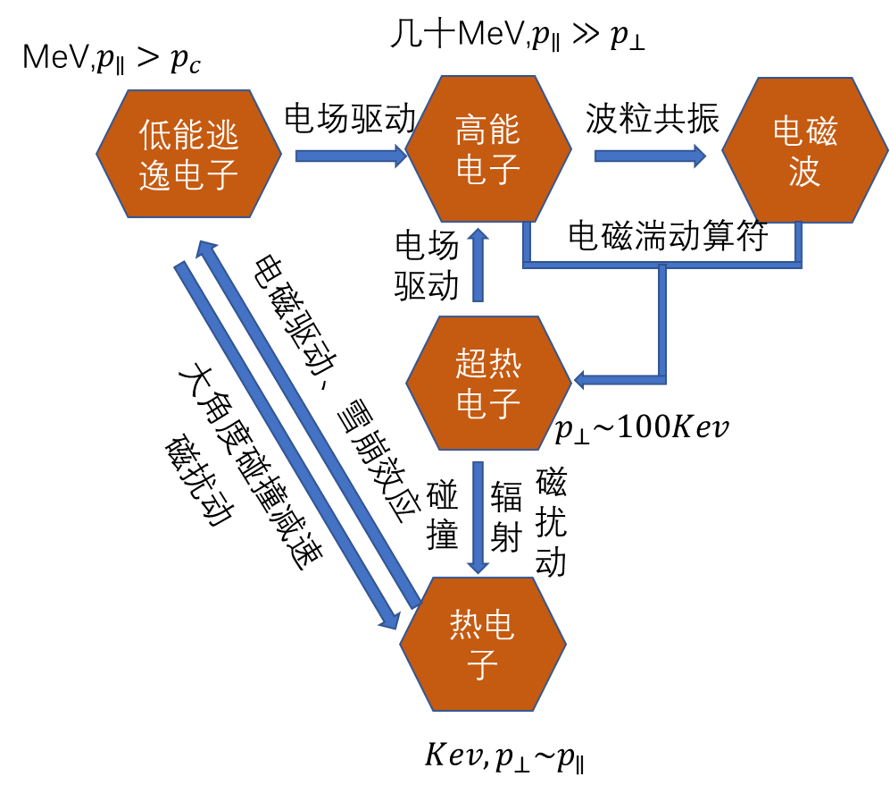
\includegraphics[width=12cm]{image39_1.png}
\caption{\label{fig:nts}非热化电子演化流程图。(注:超热电子的$p_⊥$和$p_∥$具有同等数量级\cite{RN2031},能量可达到百keV,高能电子投掷角几乎为零,但能量为MeV量级,低能逃逸电子表示电子速度和逃逸临界速度同量级,热电子表示具有热平衡分布的电子。)}
\end{figure}
\subsection{动理学分析}\label{sec:kinetic}
定量分析上述过程,必须通过动理学方程描述,其基本方程为\cite{RN1827}:
\begin{equation}
\frac{\partial f}{\partial t}-\mathrm{e} E_{\|}\left(\xi \frac{\partial f}{\partial p}+\frac{1-\xi^{2}}{p} \frac{\partial f}{\partial \xi}\right)+C[f]+\frac{\partial}{\partial \boldsymbol{p}} \cdot \boldsymbol{F}_{\mathrm{rad}} f+D[f]+L[f]=S_{A}[f]+S_{T}[f]
\end{equation}
其中e是电子电荷,$E_∥$是平行磁场的电场强度,$p=m_e γv$,$γ=1/\sqrt{1-(v/c)^2}$,$v$表示速
度,$m_e$表示电子静止质量,$ξ=p_{∥}/p$表示电子运动方向和磁力线夹角的余弦,f表示电子速度分
布函数,且$\int{f\dif^3 p}	=n_e$。$C[f]$表示Fokker-Planck碰撞算符,$F_{rad}$表示同步辐射反作用力,$D[f]$表示准线性扩散算符包括反常多普勒效应、切伦科夫效应以及多普勒效应,$L[f]$表示由于磁扰动引起的逃逸电子损失算符,$𝑆_𝐴[𝑓]$表示由于大角度碰撞导致的雪崩效应,$S_T[f]$表示电子热源项,用来补充损失的逃逸电子。Fokker-Planck碰撞算符$𝐶[𝑓]$和电场驱动项共同描述了热电子在电场驱动下变成初级逃逸电子的物理过程,对应\autoref{fig:nts}中低能逃逸电子和高能电子的形成;同步辐射算符$\frac{\partial}{\partial p}(𝑭_{rad}𝑓)$描述了超热电子以及高能电子辐射减速过程,对应\autoref{fig:nts}中辐射阻尼;准线性扩散项描述了电子和电磁波相互作用导致电子动量方向散射过程,对应\autoref{fig:nts}中电磁湍动散射过程;而雪崩算符$𝑆_A[𝑓]$则描述了超热电子和逃逸电子大角度碰撞过程,对应\autoref{fig:nts}中大角度碰撞减速和雪崩效应。至此所有的物理过程都有了对应的数学模型,下面分别介绍每一项算符:
\
\par 
\noindent
1.Fokker-Planck碰撞算符$C[f]$ \par
 Fokker-Planck碰撞算符描述的是电子通过小角度碰撞散射效应导致速度分布的变化,其方程形
式比具有普适的玻尔兹曼碰撞算符更加简单。Fokker-Planck算符建立过程中一般将粒子分为试探粒子和
主体粒子两部分,将主体粒子近似为热电子背景,试探粒子按照主体粒子的扰动处理,这时Fokker-
Planck项可以用线性算符表示为$C\{f\}=C^l\{f\}=C ̂^{tp}+C ̂^{fp}$,其中试探粒子项$C ̂^{tp} \{f_1,f_M \}$描述的是试
探粒子和主体等离子体碰撞后试探粒子速度分布的扰动,而场粒子项$C ̂^{fp} \{f_M,f_1\}$描述的是受试探
粒子碰撞后主体等离子体速度分布的扰动。当感应电场导致主体分布剧烈改变时才需要考虑非线性算符,该过程理论工作由Braams和Karney在1989年完成\cite{RN2023},并在2017年由Stahl通过计算机完成相应的
过程的数值求解\cite{RN1894}。非线性过程主用在等离子体破裂等研究上,本论文中碰撞算符所采用的方法均为线
性算符。 \par
线性碰撞算符$C ̂^{tp}[f] $可以表示为\cite{RN2025}
\begin{equation}\label{eq:tpfok}
\left.\hat{C}^{t p}=\left(v_{\mathrm{D}}^{\mathrm{ee}}+v_{\mathrm{D}}^{\mathrm{ei}}\right) \mathcal{L}\left\{f_{\mathrm{e}}\right\}+\frac{1}{p^{2}} \frac{\partial}{\partial p}\left[p^{3}\left(v_{\mathrm{S}}^{\mathrm{ee}} f_{\mathrm{e}}+\frac{1}{2} v_{\|}^{\mathrm{ee}} p \frac{\partial f_{\mathrm{e}}}{\partial p}\right)\right]\right]
\end{equation}
其中碰撞频率$\nu_D^{ee}$,$\nu_D^{ei}$ 表征电子-背景电子、电子-背景离子碰撞过程中速度方向散射
速率,$\nu_S^{ee}$描述了电子与背景电子碰撞而减速的速率,$\nu_{∥}^{ee}$表示电子平行方向速度
扩散速率,洛伦兹因子$L=1/2∂/∂ξ(1-ξ^2 )∂/∂ξ$。$\nu_S^{ee}$,$\nu_{∥}^{ee}$,$\nu_D^{ee}$以及$\nu_D^{ei}$分别为
\begin{equation}\label{eq:charnude}
\begin{aligned}
v_{\mathrm{S}}^{\mathrm{ee}} & = \frac{1}{\tau_{\mathrm{c}}} \frac{1}{p} \frac{\ln \Lambda^{\mathrm{ee}}}{\ln \Lambda_{0}} \Psi_{\mathrm{S}}(\bar{p}, \Theta) \\
v_{\|}^{\mathrm{ee}} & = \frac{1}{\tau_{\mathrm{c}}} \frac{2 \gamma \Theta}{\mathrm{p}^{3}} \Psi_{\mathrm{S}}(\bar{p}, \Theta) \\
v_{\mathrm{D}}^{\mathrm{ee}} & = \frac{1}{\tau_{\mathrm{c}}} \frac{2}{p^{2}} \frac{\ln \Lambda^{\mathrm{ee}}}{\ln \Lambda_{0}} \Psi_{\mathrm{D}}(\bar{p}, \Theta), \\
v_{\mathrm{D}}^{\mathrm{ei}} & = \frac{1}{\tau_{\mathrm{c}}} \frac{\gamma}{\mathrm{p}^{3}} \frac{\ln \Lambda^{\mathrm{ei}}}{\ln \Lambda_{0}} Z_{\mathrm{eff}}
\end{aligned}
\end{equation}
其中$\Theta=\frac{T_e}{m_ec^2}$,$Z_{eff}=\sum_j\frac{n_jZ_j^2}{n_e}$表示有效等离子体电荷数,$\tau_{\mathrm{c}}=\frac{4 \pi \varepsilon_{0}^{2} m_{\mathrm{e}}^{2} c^{3}}{n_{\mathrm{e}} e^{4}\ln \Lambda_{0}}$表示相对论碰撞时间,库伦对数分别为:
\begin{subequations}
\begin{align}
\ln \Lambda_{0} & = 14.9-0.5 \ln \left(n_{\mathrm{e}}\left[10^{20} \mathrm{~m}^{-3}\right]\right)+\ln (T[\mathrm{keV}]) \\
\ln \Lambda^{\mathrm{ee}} & = \ln \Lambda_{0}+\frac{1}{k} \ln \left(1+\left[\frac{2(\gamma-1)}{\bar{p}_{\mathrm{Te}}^{2}}\right]^{\frac{k}{2}}\right) \\
\ln \Lambda^{\mathrm{ei}} & = \ln \Lambda_{0}+\frac{1}{k} \ln \left[1+\left(\frac{2 \bar{p}}{\bar{p}_{\mathrm{Te}}}\right)^{k}\right] \\
\bar{p}_{T_{e}} & = \sqrt{\left(\frac{2 T_{e}}{m_{e} c^{2}}\right)}
\end{align}
\end{subequations}
$\ln \Lambda_0$表示热库伦对数\cite{RN1166},$lnΛ^{ee}$和$lnΛ^{ei}$为考虑相对论修正后的库伦对数,其中修正因子k取0.2,用来实现热能和高能之间平滑过渡\cite{RN1818}。$Ψ_D$和$Ψ_S$方程形式分别为:
\begin{subequations}
\begin{align}
&\Psi_{\mathrm{S}}(\bar{p}, \Theta)=\frac{\gamma^{2} \Psi_{1}-\Theta \Psi_{0}+(\Theta \gamma-1) p e^{-\frac{\gamma}{\Theta}}}{p^{2} K_{2}\left(\frac{1}{\Theta}\right)} \\
&\begin{aligned} 
\Psi_{\mathrm{D}}(\bar{p}, \Theta)= & \frac{1}{2 \gamma p^{3} K_{2}\left(\frac{1}{\Theta}\right)}\left(\left(p^{2} \gamma^{2}+\Theta^{2}\right) \Psi_{0}+\Theta\left(2 p^{4}-1\right) \Psi_{1}\right. \\ 
 &\left.+\gamma \Theta\left[1+\Theta\left(2 p^{2}-1\right)\right] p e^{-\frac{\gamma}{\Theta}}\right)
\end{aligned}
\end{align}
\end{subequations}
其中
\begin{align}
\Psi_{0}&=\int_{0}^{\bar{p}} \frac{1}{\sqrt{1+s^{2}}} \exp \left(-\sqrt{1+s^{2}} / \Theta\right) d s \\
\Psi_{1}&=\int_{0}^{\bar{p}} \exp \left(-\sqrt{1+s^{2}} / \Theta\right) d s
\end{align}
$K_2$表示第二类修正贝塞尔函数的二阶形式。
该方程描述的是分布函数在主体背景温度为$T_e$的等离子体中的演化。由于该方程只描述了试探粒子项,没有考虑主体等离子体受到试探粒子碰撞后的变化,因此该方程不满足动量守恒和能量守恒的原则。能量守恒以及动量守恒还需要考虑主体等离子体在受到试探粒子碰撞后自身分布函数的变化$C ̂^{fp}$,这方面的工作由B. Li等人在2011年完成\cite{RN1935},非相对论主体粒子碰撞项可表示为\cite{RN1809}:
\begin{equation}
\hat{C}^{\mathrm{fp}}[f]=\frac{c_{C}}{\pi^{\frac{3}{2}}} \mathrm{e}^{-\bar{v}_{\mathrm{e}}^{-2} x^{2}}\left[\frac{2 x^{2}}{\bar{v}_{\mathrm{e}}^{4}} \frac{\partial^{2} G}{\partial x^{2}}-\frac{2}{\bar{v}_{\mathrm{e}}^{2}} H+4 \pi f\right]
\end{equation}
其中G、H表示Rosenbluth势,满足关系:
\begin{align}
\tilde{\mathrm{v}}_{\mathrm{e}}^{2} \nabla_{\mathrm{v}}^{2} H &=-4 \pi f  \\
 \tilde{\mathrm{v}}_{\mathrm{e}}^{2} \nabla_{\mathrm{v}}^{2} G &=2 H
\end{align}
并且
\begin{equation*}
\begin{aligned}
\widetilde{v}_{e}&=\sqrt{\frac{2 \tilde{T}}{m}}\\
\bar{v}_{e}&=\frac{v_{e}}{\widetilde{v}_{e}}\\
 c_{C}&=\frac{3 \sqrt{\pi}}{4} \bar{v}_{e e}\\
 \bar{v}_{e e}&=\frac{v_{e e}}{\widetilde{v}_{\mathrm{ee}}}\\
\tilde{v}_{\mathrm{ee}}&=16 \sqrt{\pi} e^{4} \tilde{n} \frac{\ln \widetilde{\Lambda}}{3 m^{2} \tilde{v}_{\mathrm{e}}^{3}}\\
 c_{\xi}&=Z_{e f f}+\phi-\Psi+\frac{\bar{v}_{e}^{2} \delta^{4} x^{2}}{2}
\end{aligned}
\end{equation*}
$Z_{eff}$是有效离子电荷数,$x=v/\tilde{v_e}$表示约化速度。$Φ$和$Ψ$分别表示误差函数和钱德拉塞卡函数。实际计算中,由于我们关心的是非热化电子分布在等离子体背景中的演
化行为,而主体等离子体主要涉及电流、电阻、温度等宏观参数,这些参数在模拟中可以根据实验测量
时时更新。因此在处理非热化电子问题时,本论文中Fokker-Planck碰撞算符计算过程只考虑了试探粒子碰撞项,这样虽然失去主体等离子体的演化过程,但研究非热化电子的演化却不受影响\cite{RN1818,RN814,RN1744,RN1800,RN1815}。
\par \noindent
2.辐射阻尼算符$\frac{\partial}{\partial \boldsymbol{p}} \cdot\left(F_{\mathrm{rad}} f\right)$ \par

 在磁化等离子体中,当电子速度增加到相对论速度时,同步辐射逐渐占据主导,导致辐射阻尼直到和电场力平衡,这时候电子平行方向速度将会达到稳定点。电子回旋辐射会导致能量损失,如果垂直方向能量没有补给的话,垂直速度将会不断降低直到为零,但实际上电子和离子的散射会一直提供一部分能量给垂直方向,这样就导致垂直方向速度也存在不为零的稳定点,此时回旋辐射消耗的能量和电子离子散射获得的能量达到平衡。\par
根据A.Stahl2015年发表在PRL上的文章\cite{RN1770},同步辐射扩散项可表示为:
\begin{equation}\label{eq:radforce}
\frac{\partial}{\partial \boldsymbol{p}} \cdot\left(F_{\mathrm{rad}} f\right)=-\frac{1}{p^{2}} \frac{\partial}{\partial p}\left(\frac{\gamma p^{3}\left(1-\xi^{2}\right)}{\tau_{r}} f\right)+\frac{\partial}{\partial \xi}\left(\frac{\xi\left(1-\xi^{2}\right)}{\gamma \tau_{r}} f\right)
\end{equation}
\noindent	其中$\tau_{r}=\frac{6 \pi\left(m_{e} c\right)^{3}}{e^{4} B^{2}}$表示辐射阻尼时间尺度\cite{RN1844},B表示磁场强度。在\autoref{eq:radforce}式右边第一项表示平行方向同步辐射导致的辐射阻尼,第二项表示回旋辐射阻尼项,描述电子回旋辐射导致的角动量损失。\\
3.雪崩算符$S_A [f]$ \par
与Fokker-Planck碰撞算符描述小角度碰撞过程相反的是大角度碰撞过程,该过程的完备描述只能由最具普遍形式的玻尔兹曼碰撞算符给出。初级逃逸电子形成后,它们穿行在主体等离子体背景中时刻面临与背景电子碰撞。当大角度碰撞发生时,逃逸电子有可能会因为碰撞失去能量落入非逃逸速度区间导致逃逸速度减小,或者继续保持在逃逸速度区间,这部分的动理学描述用玻尔兹曼碰撞算符表示为$C_{ee}^B\{f_e,f_{Me}\}$,其中$f_{Me}$是一种热平衡态分布,$f_e=f_{Me}+δf_e$表示等离子体分布,分别由热平衡分布$f_{Me}$和非热平衡分布$δf_e$构成。在计算高能逃逸电子时,$f_{Me}$的速度分布区域远小于$δf_e$,因此在计算过程中将$f_{Me}$简化为$f_{Me}=n_e δ(\vp)$。另一方面,背景电子受到逃逸电子碰撞后获得的速度也有可能产生新的逃逸电子,该过程的玻尔兹曼碰撞算符为$C_{ee}^B \{f_{Me},f_e \}$。
玻尔兹曼碰撞算符利用碰撞微分截面描述了通过两体碰撞导致单位时间分布函数的变化,碰撞算符可以表示为
$C_{a b}\left(f_{a}\right)=\frac{\left(d n_{a}\right)_{c, a b}}{d t d p}$
其中$(𝑑𝑛_𝑎)_{𝑐,ab}$表示a类型的粒子和b类型的粒子碰撞后导致a类型粒子密度的变化。$(𝑑𝑛_𝑎)_{𝑐,ab}$的方程由Lifshitz \& PitaeVski(1981)\cite{RN1938}	和Cercignani \& Kremer(2002)\cite{RN1940} 给出:
\begin{equation}
\left(\mathrm{d} n_{a}\right)_{c, a b}=f_{a}\left(\boldsymbol{p}_{1}\right) f_{b}\left(\boldsymbol{p}_{2}\right) \bar{g}_{\phi} \mathrm{d} \bar{\sigma}_{a b} \mathrm{~d} \boldsymbol{p}_{1} \mathrm{~d} \boldsymbol{p}_{2} \mathrm{~d} t-f_{a}(\boldsymbol{p}) f_{b}\left(\boldsymbol{p}^{\prime}\right) g_{\phi} \mathrm{d} \sigma_{a b} \mathrm{~d} \boldsymbol{p} \mathrm{d} \boldsymbol{p}^{\prime} \mathrm{d} t
\end{equation}
右边第一项是增长项,描述的粒子a因和粒子b碰撞由动量$p_1$散射到p的速率,第二项表示损失项,描述粒子a散射偏离动量p的速率,这里引入了Møller相对速度\cite{RN2058}$g_{\phi}=\sqrt{\left(\boldsymbol{v}-\vv^{\prime}\right)^{2}-\frac{\left(\vv \times \vv^{\prime}\right)^{2}}{c^{2}}}$以及由散射过程中$\vp_1$,$\vp_2\to \vp,\vp'$微分碰撞截面$dσ_{ab}$。将$(dn_a)_{c,ab}$对时间和$\vp$微分并对速度$\vp_1$,$\vp_2$和$\vp'$积分得到碰撞算符为
\begin{equation}
C_{\mathrm{ee}}^{B}\left\{f_{\mathrm{e}}, f_{\mathrm{e}}\right\} \approx C_{\mathrm{ee}}^{B}\left\{f_{\mathrm{e}}, f_{\mathrm{Me}}\right\}+C_{\mathrm{ee}}^{B}\left\{f_{\mathrm{Me}}, f_{\mathrm{e}}\right\} \equiv C_{\text {boltz }}(\boldsymbol{p})
\end{equation}
根据O. Embréus\cite{RN1811}	的计算,雪崩算符用玻尔兹曼碰撞项的勒让德函数形式表示为
\begin{equation}
S_{A}[f]=\Sigma_{L} C_{L}(p) P_{L}(\xi)
\end{equation}
 $P_{L}(\xi) $ 表示 Legendre 函数, $ \mathrm{L}=0, \pm 1 , \pm 2 , \pm 3, \ldots$ , 该模型考虑了高能电子和 背景电子碰撞, 具体表达形式为:
\begin{align}
 &\begin{aligned}
C_{L}\left\{f_{\mathrm{e}}, f_{\mathrm{Me}}\right\} =& \frac{\left(m_{\mathrm{e}} c\right)^{-3}}{2 \tau_{\mathrm{c}} \ln \Lambda} \frac{1}{\gamma p} \int_{p_{0}}^{p^{*}} \mathrm{~d} p_{1} \frac{p_{1}^{3}}{\gamma_{1}} f_{L}\left(p_{1}\right) P_{L}\left(\xi^{*}\right) \Sigma\left(\gamma, \gamma_{1}\right) \\
- &\frac{1}{4 \tau_{\mathrm{c}} \ln \Lambda} \frac{v}{c} f_{L}(p) \int_{\gamma_{\mathrm{m}}}^{\gamma+1-\gamma_{\mathrm{m}}} \mathrm{d} \gamma_{1} \Sigma\left(\gamma_{1}, \gamma\right) 
\end{aligned} \label{eq:CLfefMe} \\ 
 &\begin{aligned}
C_{L}\left\{f_{\mathrm{Me}}, f_{\mathrm{e}}\right\}  =& \frac{\left(m_{\mathrm{e}} c\right)^{-3}}{2 \tau_{\mathrm{c}} \ln \Lambda} \frac{1}{\gamma p} \int_{p^{*}}^{\infty} \mathrm{d} p_{1} \frac{p_{1}^{3}}{\gamma_{1}} f_{L}\left(p_{1}\right) P_{L}\left(\xi^{*}\right) \Sigma\left(\gamma, \gamma_{1}\right) \\
-&\frac{\left(m_{\mathrm{e}} c\right)^{-1}}{4 \tau_{\mathrm{c}} \ln \Lambda} \delta_{L, 0} \frac{\delta(p)}{p^{2}} \int_{p_{0}\left(p_{\mathrm{m}}\right)}^{\infty} \mathrm{d} p^{\prime} \frac{p^{\prime 3}}{\gamma^{\prime}} f_{0}\left(p^{\prime}\right) \int_{\gamma_{\mathrm{m}}}^{\gamma^{\prime}+1-\gamma_{\mathrm{m}}} \mathrm{d} \gamma_{1} \Sigma\left(\gamma_{1}, \gamma^{\prime}\right) \label{eq:CLfMefe}
\end{aligned} 
\end{align}
该方程考虑了粒子的速度分布f,散射角度(这里表示为勒让德级数L)对雪崩效应的贡献,且方程自身满足了密度守恒、动量守恒和能量守恒条件。与Rosenbluth–Putvinski\cite{RN1793} 模型中假设逃逸电子速度无穷大以及Chiu–Harvey\cite{RN1941} 模型中考虑逃逸速度分布但假设逃逸电子速度的投掷角为零相比,这个模型更具完备性。\\
4.磁扰动损失算符$L[f]$\par
由于随机磁扰动造成的逃逸电子损失算符可表示为\cite{RN2076,RN2086}:
\begin{equation}
\begin{aligned}
L[f] & = -\frac{f}{\tau_{\delta B}} \\
\tau_{\delta B} & = \frac{(r-a)^{2}}{4\left|v_{\|}\right| D_{s t}} \gamma^{5} \\
D_{s t} & = \pi R_{\text {eff }}\left(\frac{\delta B_{r}}{B}\right)^{2} \\
R_{e f f} & = R q \pi 
\end{aligned}\label{eq:Harvey}
\end{equation}
其中R表示装置大半经,a表示装置小半径,r表示小半径位置,q表示安全因子,$𝑣_{∥}$表示速度,$𝛾$表示洛伦兹因子。\\
5.电子热源项$S_T[f]$\par
\begin{equation}
{S}_T[f]=\alpha f_m
\end{equation}
其中$α=1-∫4πp^2 F_0 dp$ ,$α$表示添加的热等离子体系数以弥补由于逃逸电子造成的密度损失,$f_M$为归一化热电子分布,$F_0$为分布函数n=0的勒让德系数。\\
6.电磁波散射算符$D[f]$\par
在冷等离子体近似中,磁化等离子体中的色散方程用磁流体模型计算给出。我们可以获通过色散方程获得等离子体中存在的各种本征波,例如阿尔芬波、非寻常波、哨声波、磁声波等、朗缪尔波等。如果考虑非热化电子成分,根据动理学方程中介电常数和分布函数的关系,等离子体可以通过共振的形式激发(或阻尼)本征电磁波,而激发出的电磁波又会反作用于等离子体自身,该过程称为电磁湍动过程\cite{胡希伟2006等离子体理论基础}。\par
为了研究电磁湍动过程,首先需要建立分布函数和电磁波增长率之间的关系,常见的处理方法是将分布函数分成两部分,一部分是冷等离子体部分,该部决定等离子体波的色散关系$\omega=\omega(k,r)$,另一部分为非热化电子分布,这部分的分布函数决定波增长率大小,当增长率远小于频率时,$\omega_r≫\omega_i$,增长率可以通过对等离子体色散关系线性化处理,由一阶扰动展开得到\cite{RN1452}:
\begin{equation}\label{eq:gamma}
\Gamma_{v}=-i \frac{E_{\alpha}^{*} E_{\beta} \omega^{2} \varepsilon_{\alpha \beta}^{A}}{E_{\alpha}^{*} E_{\beta} \frac{\partial}{\partial \omega} \omega^{2} \varepsilon_{\alpha \beta}^{H}}
\end{equation}
增长率包含等离子体会电张量  $\epsilon_{\alpha \beta}$, $\alpha$ 、 $\beta$表示$  \mathrm{x} $、 $\mathrm{y} $、$ \mathrm{z} $ 三个方向电场矢量,  $\epsilon_{\alpha \beta} $ 一般 是复数形式, $ \epsilon_{\alpha \beta}=\epsilon_{\alpha \beta}^{H}+i \epsilon_{\alpha \beta}^{A}$ , 具体推导在 T.H.Six 书 《WAVES in PLASMAS》\cite{RN1836}中给出了详细的过程, 这里只给出其最终结果:
\begin{subequations}\label{eq:disper}
\begin{align}
&\varepsilon_{x x} = \varepsilon+\frac{4 \pi e^{2}}{\omega} \int d^{3} p \sum_{n = -\infty}^{\infty} A_{n} \frac{n^{2} \omega_{c e}^{2}}{k_{\perp}^{2}} J_{n}^{2} \\
&\varepsilon_{x y} = -\varepsilon_{y x} = i g+i \frac{4 \pi e^{2}}{\omega} \int d^{3} p \sum_{n = -\infty}^{\infty} A_{n} \frac{n \omega_{c e} V \sin \theta}{k_{\perp}} J_{n} J_{n}^{\prime} \\
&\epsilon_{y y} = \varepsilon+\frac{4 \pi e^{2}}{\omega} \int d^{3} p \sum_{n = -\infty}^{\infty} A_{n} V^{2} \sin ^{2} \theta J_{n}^{\prime 2} \\
&\varepsilon_{x z} = \varepsilon_{z x} = \frac{4 \pi e^{2}}{\omega} \int d^{3} p \sum_{n = -\infty}^{\infty} B_{n} \frac{n \omega_{c e} V \cos \theta}{k_{\perp}} J_{n}^{2} \\
&\varepsilon_{y z} = -\varepsilon_{z y} = -i \frac{4 \pi e^{2}}{\omega} \int d^{3} p \sum_{n = -\infty}^{\infty} B_{n} V^{2} \sin \theta \cos \theta J_{n} J_{n}^{\prime} \\
&\varepsilon_{z z} = \eta+\frac{4 \pi e^{2}}{\omega} \int d^{3} p \sum_{n = -\infty}^{\infty} B_{n} V^{2} \cos ^{2} \theta J_{n}^{2}
\end{align}
\end{subequations}
\noindent	其中
\begin{equation*}
\begin{aligned}A_{n}= & \frac{1}{\left(\omega-k_{\|} \mathrm{V} \cos \theta-n \omega_{\mathrm{ce}}\right)} \\& \times\left[\frac{1}{V} \frac{\partial f}{\partial p}+\frac{\omega \cos \theta-k_{\|} V}{\omega \mathrm{pV} \sin \theta} \frac{\partial f}{\partial \theta}\right] \\B_{n}= & \frac{1}{\left(\omega-k_{\|} \mathrm{V} \cos \theta-n \omega_{\mathrm{ce}}\right)} \\& \times\left[\frac{1}{V} \frac{\partial f}{\partial p}+\frac{1}{\mathrm{pV} \cos \theta}\left(\frac{n \omega_{\mathrm{ce}}}{\omega \sin \theta}-\sin \theta\right) \frac{\partial f}{\partial \theta}\right]\end{aligned}
\end{equation*}
并且
\begin{equation*}
\begin{aligned}
\varepsilon& \equiv 1-\sum_{e ; i} \frac{\omega_{\mathrm{p}}^{2}}{\omega^{2}-\omega_{\mathrm{c}}^{2}} \\
g &\equiv-\sum_{e ; i} \frac{\omega_{\mathrm{c}}}{\omega} \frac{\omega_{\mathrm{p}}^{2}}{\omega^{2}-\omega_{\mathrm{c}}^{2}}  \\
\eta &\equiv 1-\sum_{e ; i} \frac{\omega_{\mathrm{p}}^{2}}{\omega^{2}} \\\omega_{c e} = \frac{\omega_{c}}{\gamma}, \omega_{c0} &= \frac{-e B}{m_{e}}, \gamma  = \sqrt{1+\left(\frac{p}{m c}\right)^{2}}
\end{aligned}
\end{equation*}
其中被积函数存在奇点,根据Sokhotski-Plemelj理论\cite{RN1837},
\begin{equation}
\frac{1}{\omega-k_{\|} V \cos \theta-n \omega_{\mathrm{cb}}}=P\left(\frac{1}{\omega-k_{\|} V \cos \theta-n \omega_{\mathrm{cb}}}\right)+i \pi \delta\left(\omega-k_{\|} V \cos \theta-n \omega_{\mathrm{cb}}\right)
\end{equation}
P表示积分主值,将\autoref{eq:disper}代入\autoref{eq:gamma},考虑冷等离子体条件得到最终增长率方程为\cite{RN1452}:
\begin{equation}\label{eq:gammab}
\begin{aligned}\Gamma_{\mathrm{b}}= & {4 \pi^{2} e^{2} \int \mathrm{d}^{3} p \sum_{n=-\infty}^{\infty} Q_{n} } \\& \times\left[V \frac{\partial f}{\partial p}+\frac{V}{p} \frac{n \omega_{\mathrm{cb}}-\omega \sin ^{2} \theta}{\omega \cos \theta \sin \theta} \frac{\partial f}{\partial \theta}\right] \\& \left.\times \delta\left(\omega-k_{\|} \mathrm{V} \cos \theta-n \omega_{\mathrm{cb}}\right)\right]\left[\left(E_{x}^{2}-E_{y}^{2}\right) \frac{1}{\omega} \frac{\partial}{\partial \omega} \omega^{2} \varepsilon\right. \\& \left.+2 i E_{y} \frac{1}{\omega} \frac{\partial}{\partial \omega} \omega^{2} g+E_{z}^{2} \frac{1}{\omega} \frac{\partial}{\partial \omega} \omega^{2} \eta\right]^{-1} \\Q_{n} \equiv & \left\{\frac{n \omega_{\mathrm{cb}}}{k_{\perp} V} J_{n} E_{x}+E_{z} \cos \theta J_{n}+i E_{y} \sin \theta J_{n}^{\prime}\right\}^{2}\end{aligned}
\end{equation}
至此,我们获得了电磁波能量演化的微分方程:
\begin{align}
\frac{d \mathcal{E}_{k}(t)}{d t} & = 2 \Gamma_{\mathrm{b}} \mathcal{E}_{k}(t) \\
\mathcal{E}_{k}(t) & = \frac{\epsilon_{0}}{2}\left|E_{k}(t)\right|^{2}
\end{align}
以上介绍了电磁波的产生过程,那么等离子体是如何和电磁波相互作用的呢?这个问题从求解弗拉索夫方程出发:
\begin{equation}\label{eq:vlasov}
\frac{\partial f}{\partial t}+\mathrm{v} \cdot \nabla f+\frac{q}{m} \nabla_{\mathrm{p}} \cdot\left[\left(\mathbf{E}+\frac{\mathbf{v} \times \mathbf{B}}{c}\right) f\right]=0
\end{equation}
其中$∇_p$表示$∂/∂p$.求解该方程中需要用到准线性理论,在准线性理论中有三点假设需要满足:1电磁波的扰动足够小使得线性分析时利用电子未扰动轨道积分依然成立;2电磁波的增长率(衰减率)$ω_i≪ω_r$;3电磁波具有稠密的谱分布使得在等离子体状态演化的时间尺度内任何相干波之间都会因为相混而被破坏。基于这些假设,我们可以将速度分布函数分为$f=f_0+f_1$,其中$f_0$表示零阶量,$f_1$表示一阶量。为了将\autoref{eq:vlasov}表示成准线性形式,我们以电磁波空间和时间周期为积分长度,对\autoref{eq:vlasov}速度空间回旋角和时间积分:
\begin{equation}\label{eq:valsovf0}
\begin{aligned}
\frac{\partial f_{0}}{\partial t} & = -q\left <\int_{0}^{2 \pi} \frac{d \phi}{2 \pi} \nabla_{\mathbf{p}} \cdot\left[\left(\mathbf{E}^{(1)}+\frac{\mathbf{v} \times \mathbf{B}^{(1)}}{c}\right) f^{(1)}\right]\right> \\
\quad & = -\lim _{V \to \infty} q  \int \frac{d^{3} \mathbf{k}}{V} \int_ {0}^{2 \pi} \frac{d \phi}{2 \pi} \nabla_{\mathbf{p}} \cdot\left[\left(\mathbf{E}_{k}+\frac{\mathbf{v} \times \mathbf{B}_{k}}{c}\right) f_{-k}\right]
\end{aligned}
\end{equation}
根据一阶近似条件
\begin{equation}
\left(\frac{d f_{1}}{d t}\right)_{0}=-\mathrm{q}\left(\mathbf{E}_{1}+\frac{\mathrm{v}}{c} \times \mathbf{B}_{1}\right) \cdot \frac{\partial f_{0}}{\partial \mathbf{p}}
\end{equation}
其中下标0表示$f^{(1)}$沿未扰动轨道(r,p,t)空间的变化率,通过积分可得到$f^{(1)}$的方程形式为
\begin{equation}\label{eq:valsovf1}
f_{1}(\mathbf{r}, \mathbf{v}, t)=-\mathrm{q} \int_{-\infty}^{t} d t^{\prime}\left[\mathbf{E}_{1}\left(\mathbf{r}^{\prime}, t^{\prime}\right)+\frac{\mathbf{v}^{\prime}}{c} \times \mathbf{B}_{1}\left(\mathbf{r}^{\prime}, t^{\prime}\right)\right] \cdot \frac{\partial f_{o}\left(\mathbf{p}^{\prime}\right)}{\partial \mathbf{p}^{\prime}}
\end{equation}
对\autoref{eq:valsovf1}空间傅里叶变换后代入\autoref{eq:valsovf0},并将$B_k$表示成$E_k$形式 ,微分算符写为
\begin{equation}
\nabla_{p}=\vec{e}_{\rho} \frac{\partial}{\partial p_{\perp}}+\vec{e}_{\|} \frac{\partial}{\partial p_{\|}}
\end{equation}
这里默认了回旋方向均匀分布,因此忽略了$
\vec{ e}_ϕ  1/p_⊥    ∂/∂ϕ$这一项。通过繁琐的迭代运算,电磁波和等离子体湍动扩散方程最终可表示为\cite{RN1757,RN1815,RN1836,RN1829}
\begin{equation}\label{eq:emwdiffuse}
\frac{\partial f}{\partial t}=\frac{\pi e^{2}}{m_{e 0}^{2} c^{2}} \sum_{n=-\infty}^{\infty} \int d^{3} k \widehat{\Pi} p_{\perp} \delta\left(\omega_{k}-n \Omega-\frac{k_{\|} p_{\|} c}{\gamma}\right) \times\left|\psi_{n, k}\right|^{2} p_{\perp} \widehat{\Pi} f
\end{equation}
其中算符
\begin{equation}
\widehat{\Pi}=\frac{\omega_{k}-\frac{k_{\|} p_{\|} c}{\gamma}}{w_{k} p_{\perp}} \frac{\partial}{\partial p_{\perp}}+\frac{k_{\|} c}{w_{k} \gamma} \frac{\partial}{\partial p_{\|}}
\end{equation}
无量纲动量$p=p_0/mc$,$Ω=ω_{ce}/γ<0$,将 $\hat{Π}$ 转化为$(p,ξ)$坐标得
\begin{equation}
\widehat{\Pi}=\frac{1}{p} \frac{\partial}{\partial p}-\frac{w_{k} \xi-k_{\|} v}{w_{k} p^{2}} \frac{\partial}{\partial \xi}
\end{equation}
其中$p=\sqrt{p_⊥^2+p_∥^2},ξ=p_{∥}/p$ 。能量谱分布$\left|\psi_{n,k}\right|^2$\cite{RN1757} 为:
\begin{equation}\label{eq:Psi}
\left|\Psi_{n, k}\right|^{2}=\left|E_{k x} \frac{n}{z} J_{n}+i E_{k y} J_{n}^{\prime}+\frac{p_{\mid}}{p_{\perp}} E_{k z} J_{n}\right|^{2}
\end{equation}
这里$J_n$表示n阶第一类贝塞尔函数,其中的自变量是$z=(k_⊥ p_⊥ c)/ω_{ce}$ ,利用冷等离子体色散关系得到电场的极化方向为:
\begin{equation}\label{eq:polar}
\begin{pmatrix}
 E_{kx}\\
  E_{ky}\\
E_{kz}
\end{pmatrix}=\begin{pmatrix}
 1\\
 i \frac{\omega_{p e}^{2} \omega_{c e} / \omega_{\mathrm{k}}}{\omega_{\mathrm{k}}^{2}-k^{2} c^{2}-\omega_{c e}^{2}-\omega_{p e}^{2}+k^{2} c^{2} \omega_{c e}^{2} / \omega_{\mathrm{k}}^{2}}\\
\frac{k_{\|} k_{\perp} c^{2}}{\omega_{p e}^{2}+k_{\perp}^{2} c^{2}-\omega_{\mathrm{k}}^{2}}
\end{pmatrix}
\end{equation}
将\autoref{eq:polar}其带入到\autoref{eq:Psi}得:
\begin{equation}
\left|\psi_{n, k}\right|^{2}=\left|E_{k x}\right|^{2}\left|\frac{n J_{n}}{z}+\frac{\frac{J_{n}^{\prime} \omega_{p e}^{2} \omega_{c e}}{\omega_{k}}}{\omega_{k}^{2}-k^{2} c^{2}-\omega_{c e}^{2}-\omega_{p e}^{2}+\frac{k^{2} c^{2} \omega_{c e}^{2}}{\omega_{k}^{2}}}+\frac{p_{\|}}{p_{\perp}} \frac{k_{\|} k_{\perp} c^{2} J_{n}}{\omega_{p e}^{2}+k_{\perp}^{2} c^{2}-\omega_{k}^{2}}\right|^{2}
\end{equation}
关于准线性湍动过程, 我们可以通过微分算符 $ \widehat{\Pi}=\frac{\omega_{k} -\frac{k_{\|} p_{\|}{c }}{\gamma}}{w_{k} p_{\perp}} \frac{\partial}{\partial p_{\perp}}+\frac{k_{\|} c}{w_{k} \gamma} \frac{\partial}{\partial p_{\|}}$ 研究其物 理特征, 在不考虑相对论效应的情况下, 微分算符可以表示为  $\widehat{\Pi}=(1-   \left.\frac{\mathrm{k}_{\|} v_{\|}}{w_{k r}}\right) \frac{1}{p_{\perp}} \frac{\partial}{\partial p_{\perp}}+\frac{k_{\|} v_{\perp}}{w_{k} p_{\perp}} \frac{\partial}{\partial p_{\|}}$ , 其对应的特征线方程满足
\begin{equation}\label{eq:sf}
v_{\perp}^{2}+\left(v_{\|}-\frac{\omega_{k r}}{k_{\|}}\right)^{2}=\xi
\end{equation}
特征线的物理意义是描述物理量扰动的传播方向,数学上是将偏微分方程化为常微分方程\cite{RN2028},这里我们用特征线研究分布函数的演化方向。
\par 关于准线性湍动方程的特征线,Thomas Howard Stix 在著作《WAVES IN PLASMAS》\cite{RN1836}中有一段精彩的描述,书中优美地结合了量子力学和能量守恒定理,对特征线方程所包含的物理给出了精妙绝伦的解释,这里摘录如下:根据相对论理论,物质的能量为$E^2=m_0^2 c^4+p^2 c^2$,我们可以得到$EδE=c^2 p∙δp$,因此有$δE=v∙δp$(其中$c^2 p/E=v,E=γmc^2,p=γmv) $。同时根据量子力学理论,当粒子吸收一个光子能量$ΔE=ℏω_k$后,根据动量守恒,粒子平行方向动量变化为$δp_{∥}=ℏk_{∥}$,平行方向能量变化为$δE_∥=v_∥ δp_∥=v_∥ ℏk_∥$,然后$δE=(δE/(δE_∥ ))δE_∥=(w_k/(k_∥ v_∥ )) v_∥ δp_∥$,原方程$δE=v∙δp$即可表示为
\begin{equation}\label{eq:dsf}
0=v_{\perp} \delta p_{\perp}+\left(1-\frac{\omega_{k}}{k_{\|} v_{\|}}\right) v_{\|} \delta p_{\|}
\end{equation}
在非相对论情况下,对方程\autoref{eq:dsf}积分立刻得到特征线方程\autoref{eq:sf},这也说明了为什么特征线是粒子速度的演化方向。
这个描述很好的解释了方程背后所包含的物理意义,分别从经典电磁学和量子力学得到统一的特征线方程。

等离子体中电子在均匀背景静电场作用下经过一定时间后速度分布等高线如\autoref{fig:difuvec}所示。考虑频率为$\omega$,平行方向波数为$k_z$的波在电子回旋频率为$\omega_{ce}$的等离子体中传播,则特征线的形状是以$(\frac{ω}{k_{z}} ,0)$为圆心的同心圆,分布函数梯度 $-∇_v f$沿着圆的切线方向的投影表示特征线上存在分布梯度的粒子会沿着圆的切线方向扩散,使特征线上速度分布趋于均匀。值得注意的是,由于\autoref{eq:emwdiffuse}中狄拉克函数的存在,只有共振的粒子才会被散射。我们考虑三种共振,取n=-1、0、1,我们得到三种共振速度,分别是反常多普勒共振切伦科夫共振(或朗道共振)以及多普勒共振,对应得共振速度分别是$v_{ade}=(ω+|ω_{ce} |)/k_z $,$v_{landau}=ω/k_z $和$v_{nde}=(ω-|ω_{ce} |)/k_z$ ,只有共振线附近的粒子才能参与共振。这三种共振对应不同的物理现象,我们可以通过这张图直观地描述其物理图像:1.对于多普勒共振(NDE),在密度梯度的驱动下,共振粒子将会沿着该位置圆的右上方切线方向运动,导致粒子平行方向速度和垂直方向速度同时增加,例如应电子回旋共振可利用这种机制实现对等离子体的加热和电流驱动(当然Fisch机制目前认为是是驱动电流的主要机制\cite{RN2131})。2.对于朗道共振(Landau),由于共振位置处在特征线圆的顶点位置,因此该位置的密度梯度将会驱动粒子平行方向运动,以抹平共振速度附近电子速度分布的不均匀性。3.对于反常多普勒共振(ADE),在梯度驱动下,粒子将会沿着特征线切线的左上方运动,这意味粒子在反常多普勒共振下平行方向速度减小而垂直方向速度将会增加。这里我们做一个大胆的猜想,反常多普勒共振线会导致粒子平行方向速度减速,垂直方向增大,那么这样的共振线像不像一座堤坝?粒子加速至共振速度被减速‘反弹’,同时垂直方向速度增大。粒子减速脱离共振后,又会在静电场作用下加速,又一次和共振速度相遇,然后又重复上述过程。这样周而复始,粒子是不是就像是遇到了堤坝,平行方向速度出现了阈值,垂直方向速度‘水位’不断升高?这种现象在第四章粒子模拟中得到了验证。
\begin{figure}
\centering
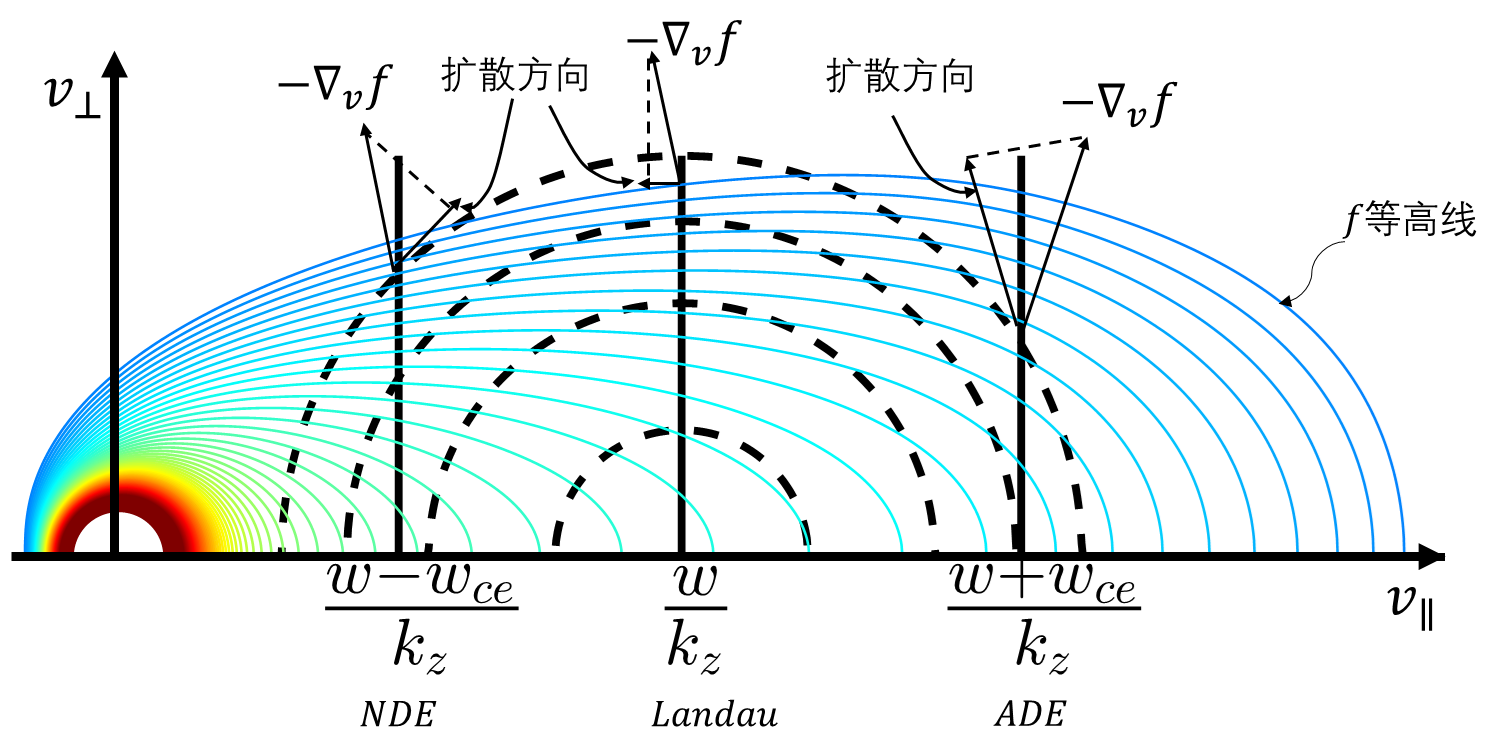
\includegraphics[width=14cm]{image40_1.png}
\caption{\label{fig:difuvec}特征线及多普勒共振、朗道共振与反常多普勒共振对应的电子速度扩散方向,其中虚线表示不同共振能量所在的特征线,只有与共振速度相交的位置才会出现动量散射}
\end{figure}\par

\section{非热化电子诊断方法 }

托卡马克中电子在磁场中运动会受到磁场的洛伦兹力,和周围电子离子的库伦力,以及感应电场对电子的静电力,绕大环方向运动的向心力等。这些力作用在电子上使电子具有丰富的运动状态,导致电子具有轫致辐射、电子回旋辐射、同步辐射等特征,不同能量的电子偏向不同的辐射类型。
\begin{figure}[ht]
\centering
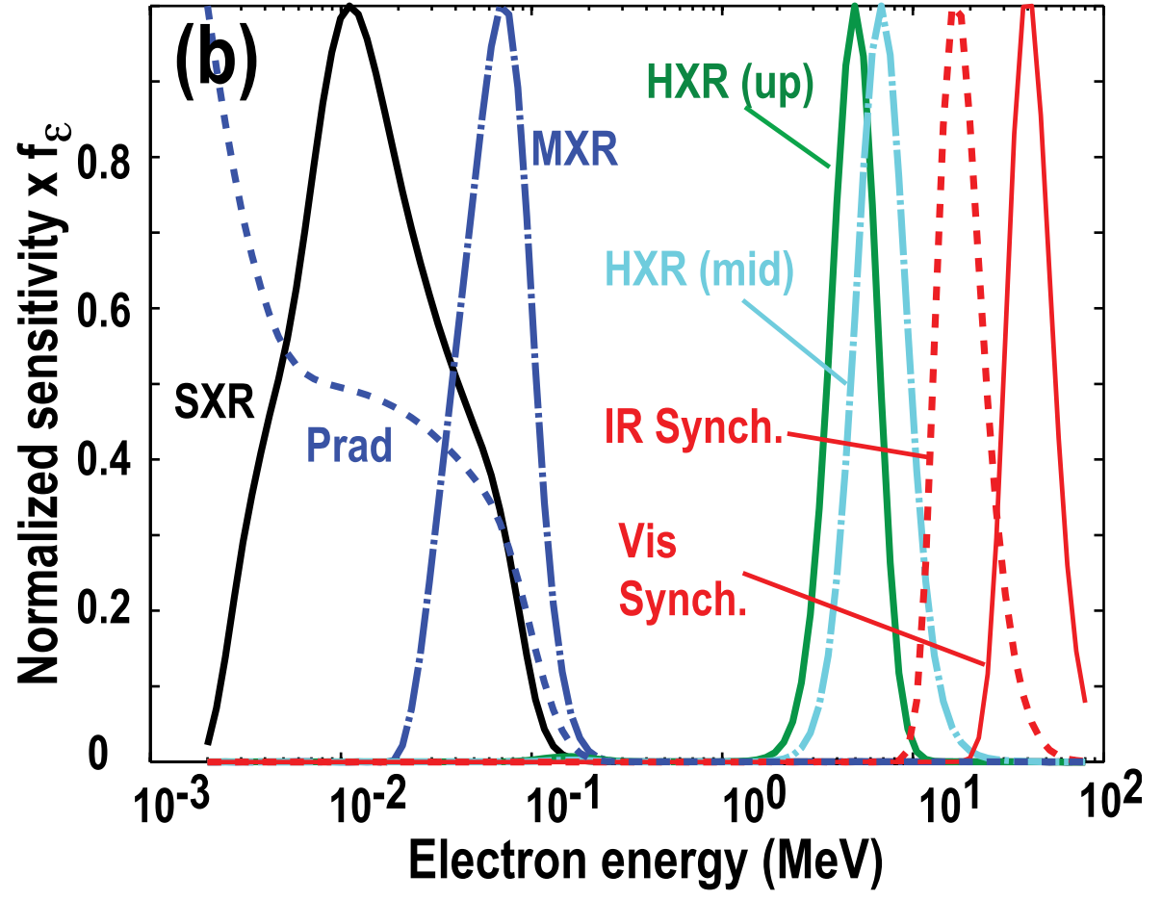
\includegraphics[width=12cm]{image41.png}
\caption{\label{fig:spec}不同辐射诊断对应的电子能量探测区间,图片来自\cite{RN1435}}
\end{figure}\par
尽管托卡马克中电子能量会由于辐射和约束能力而存在上限,非热化电子能量覆盖范围却可以从经典放电中热电子的几keV到逃逸电子中十几MeV,如此宽的能量覆盖范围导致一种诊断不能把非热化电子的速度分布特征诊断清楚。由于非热化电子的辐射谱强度分布和其携带能量有关,具有动能MeV电子的轫致辐射谱主要处在软X射线和硬X射线波段\cite{RN972},毫米波波段可以用来诊断垂直磁场方向能量keV到百keV的非热化电子\cite{RN1356},而几十MeV的高能逃逸电子在环向弯曲磁场中的加速运动产生的同步辐射主要处在红外波段以及可见光波段\cite{RN973,RN956}。因此不同能量的电子具有不同的辐射特征,相应的诊断方法也不相同。如\autoref{fig:spec}所示,其中SXR表示软X射线辐射诊断,用来诊断能量在2-10~keV的电子,Prad表示热辐射诊断用来诊断能量在100~keV以下能量的电子,MXR表示Mid X-ray辐射诊断,用来诊断能量在20-100~keV区间的电子,HXR表示硬x射线诊断,用来分析能量在1-10~MeV区间的逃逸电子,IR远红外段诊断用于分析动能在10-50~MeV的逃逸电子,而Vis Synch表示可见光波段诊断,用于诊断能量区间在30~MeV以上的逃逸电子\cite{RN1435}。
\subsection{轫致辐射诊断}
轫致辐射是托卡马克中最广泛用于诊断逃逸电子或非热化电子的诊断工具之一。轫致辐射是带电粒子与原子或原子核发生碰撞导致速度急剧改变发出的辐射。当逃逸电子被等离子体离子散射时,它的轫致辐射可以认为是“薄靶”的体轫致辐射,通过观测这些辐射可以获得逃逸电子能量信息;当逃逸电子轰击等离子体偏滤器/限制器时,它的轫致辐射相当于是“厚靶”的表面轫致辐射\cite{RN1744}。轫致辐射谱具有连续分布的特征,根据频率一般分为软X射线波段和硬X射线波段。
在软 X射线能段(光子能量1-30keV),通常采用半导体探测器,如EAST上软X射线能谱诊断[128](Soft X-ray pulse height analyzer, SXPHA)采用的是硅漂移探测器(Silicon Drift Detector,SSD)。其原理是入射X光被SSD吸收并激发电子空穴对,在探测器的偏压电场作用下形成原始电流,原始电流信号经过放大器后形成振幅正比于入射X射线能量的脉冲电压信号,脉冲电压信号进入多道分析仪(Multi-Channel Analyzer,MCA)处理成数字信号获得X射线能谱分布。如\autoref{fig:Xray}(b)为EAST放电过程中由SXPHA测得的能谱分布,由于光子能量在1-30keV区间的软X射线辐射基本都是低能量电子辐射谱(部分由杂质中性原子激发退激发过程产生的线辐射频率也在这个区间,如Ar的Ka谱,Ti的Ka谱等),低能量的电子速度分布通常假设具有热分布特征,因此通过能谱图可以拟合出电子的热温度,如\autoref{fig:Xray}(c)(d)所示。
\begin{figure}[ht]
\centering
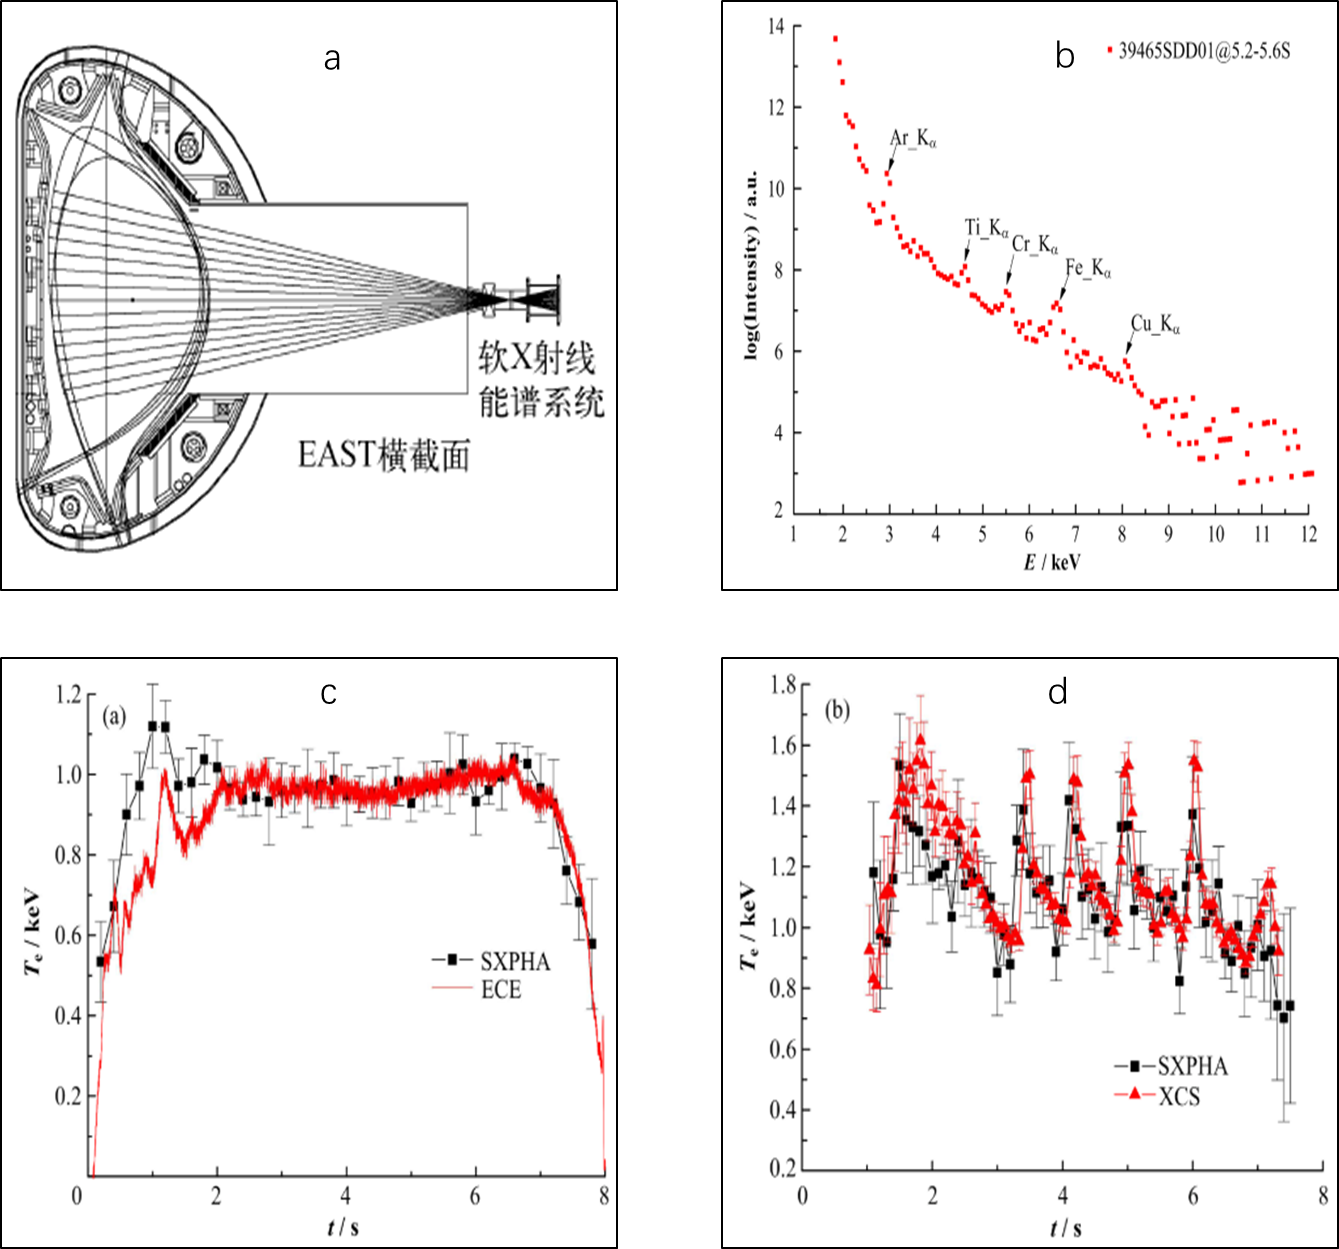
\includegraphics[width=12cm]{image42.png}
\caption{\label{fig:Xray}(a)EAST装置上SXPHA诊断空间布局(b)\#39465炮在5.2-5.6时刻软X射线能谱(c)SXPHA获得电子温度与ECE 辐射温度对比(d)SXPHA所测电子温度与弯晶谱仪所测电子温度对比(图片来自\cite{RN1491})}
\end{figure}\par
  硬X射线诊断中,垂直快电子轫致辐射诊断\cite{RN6}(Fast electron bremsstrahlung diagnostic,FEB)主要用来分析电子垂直方向能量处在30-300keV区间的电子。2018年,华中科技大学J-TEXT托卡马克装置上利用垂直FEB诊断实现了对放电初期间逃逸电子不稳定性的观测\cite{RN6}。该诊断采用CdZnTe 探测器,相对于传统Si和高纯锗等传统半导体探测器,CdZnTe作为一种新型半导体探测器具有体积小,室温可用,分辨率高等优良品质。通过合适的光路设置,如\autoref{fig:JTEXT},FEB可以实现对非热化电子空间分布的探测。除此之外,用于硬X射线能谱诊断还有碘化钠(NaI)闪烁体阵列\cite{RN956}、碲化镉(CdTe)探测器阵列\cite{RN957}	等,这里不再一一赘述。  
\begin{figure}[ht]
\centering
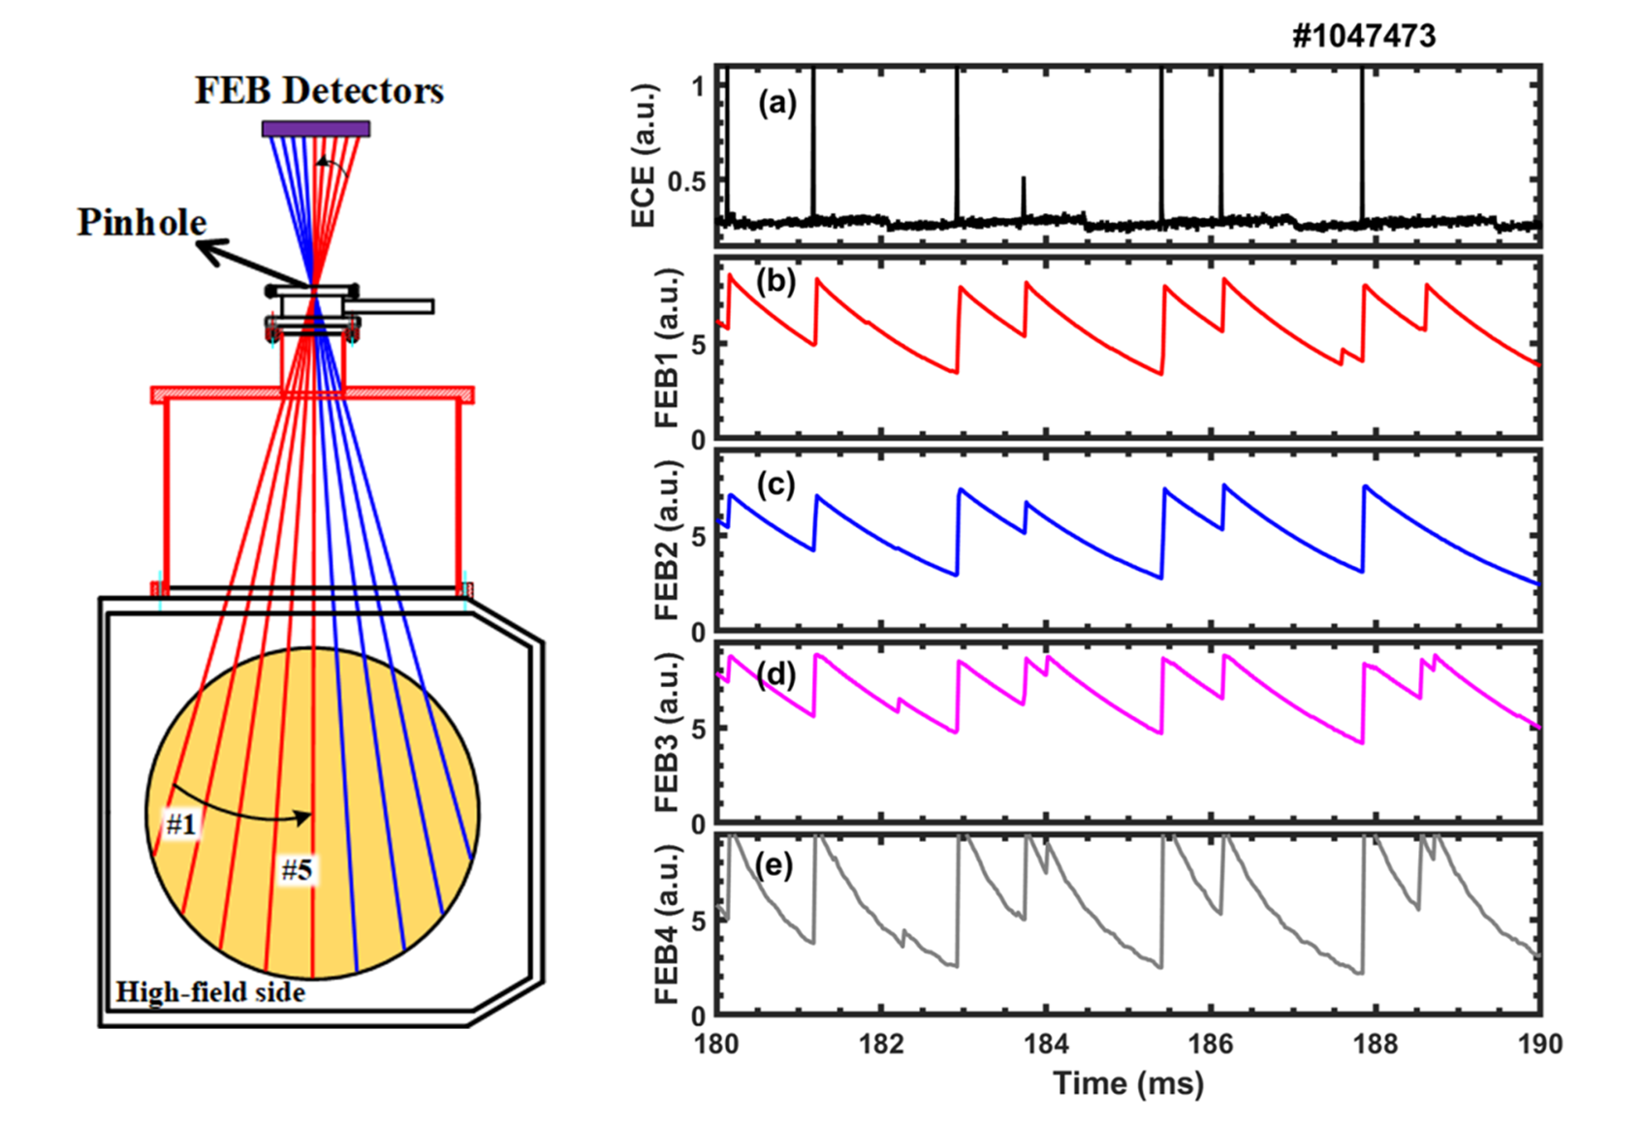
\includegraphics[width=12cm]{image43.png}
\caption{\label{fig:JTEXT}左图为J-TEXT上FEB诊断光学设置,右图表示J-TEXT放电中观测到的ECE辐射信号和FEB信号\cite{RN6}}
\end{figure}
%\clearpage
\subsection{同步辐射诊断}
 在托卡马克领域,“同步辐射”通常指的是磁场中相对论性电子的光辐射,主要取决于电子的动能和螺旋角\cite{RN990},而“回旋辐射”指的是磁场中的非相对论性电子的光辐射,主要取决于电子垂直方向的动能。如\autoref{fig:synchrotron1},同步辐射具有高能量、定向性特征,辐射角锥主要沿着电子运动方向,探测器接收光路只有沿着电子运动方向才能观测到。因此探测相机接收光路一般都在中平面沿着托卡马克环向方向,例如EAST 可见光相机(\autoref{fig:synchrotron2}(a))\cite{RN1885}和TEXTOR远红外光相机(\autoref{fig:synchrotron2}(b))\cite{RN1878}	等。
\begin{figure}[ht]
\centering
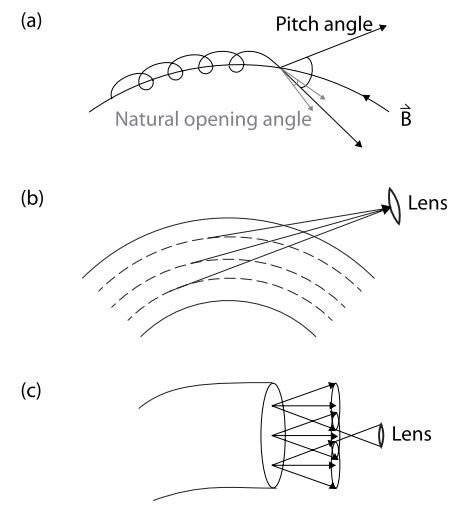
\includegraphics[width=12cm]{image44.png}
\caption{\label{fig:synchrotron1}(a)逃逸电子的同步辐射运动的俯仰角和同步辐射的辐射开口角度(b)托卡马克环向切面,不同磁面逃逸电子辐射方向(c)极向切面:来自不同区域的逃逸电子发出的同步辐射。只有在发射锥内的同步辐射被透镜收集。图片来自\cite{RN1878}}
\end{figure}

\begin{figure}[ht]
\centering
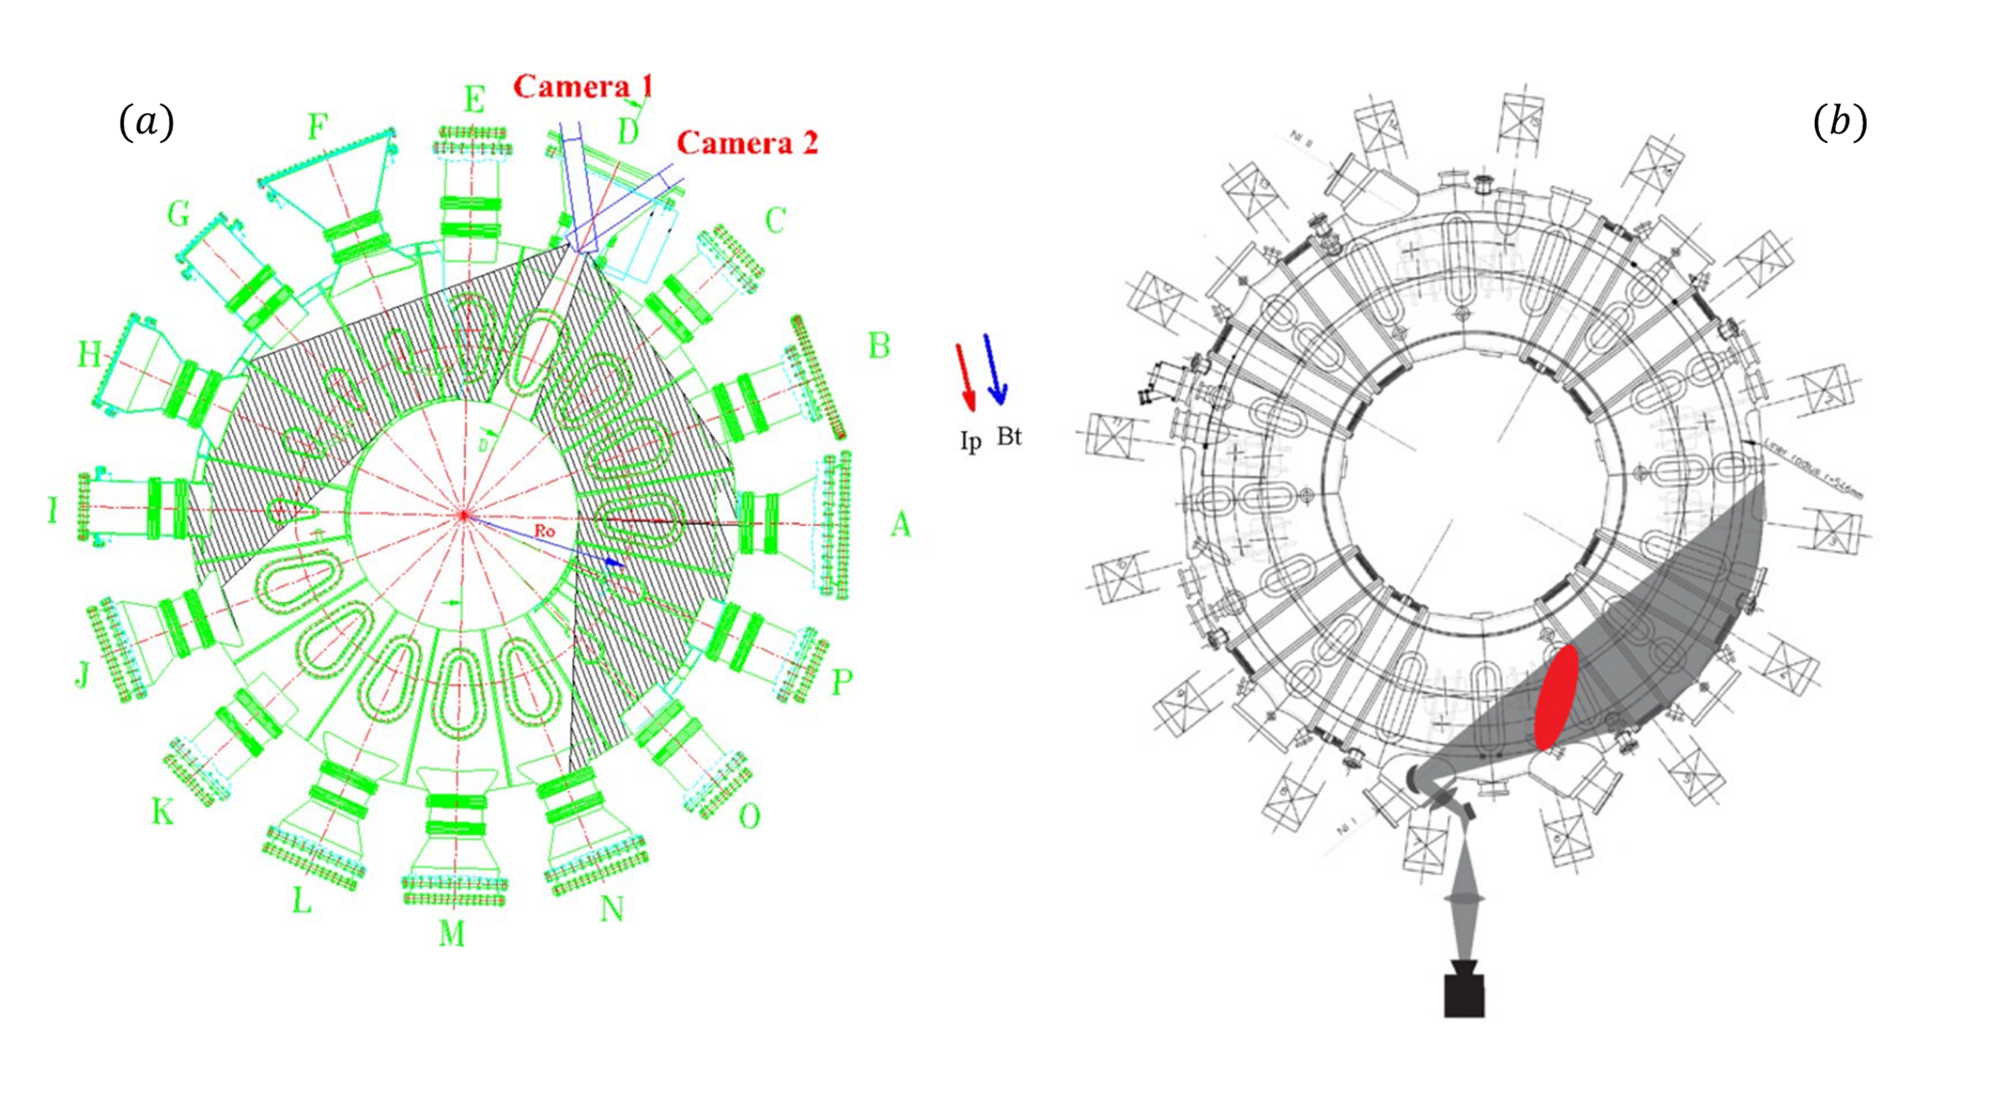
\includegraphics[width=12cm]{image45.png}
\caption{\label{fig:synchrotron2}(a)EAST装置可见光相机位置示意图\cite{RN1885}。(b)TEXTOR装置远红外相机示意图。灰色阴影区域表示接收光路区域\cite{RN1878}	}
\end{figure}
根据同步辐射方程\cite{RN1886},我们可以获得不同能量的逃逸电子对应的辐射波段。如\autoref{fig:synchrotron3}, 对于电子能量为25MeV的逃逸电子,同步辐射主要落在2-4um波段。结合同步辐射的定向性特征,可以通过沿托卡马克环向方向红外成像\cite{RN995,RN994,RN992}能获得逃逸电子的位置分布信息。\autoref{fig:synchrotron4}所展示的是EAST放电过程中不同时刻逃逸电子辐射光斑通过远红外相机成像\cite{RN1879}。
\begin{figure}[ht]
\centering
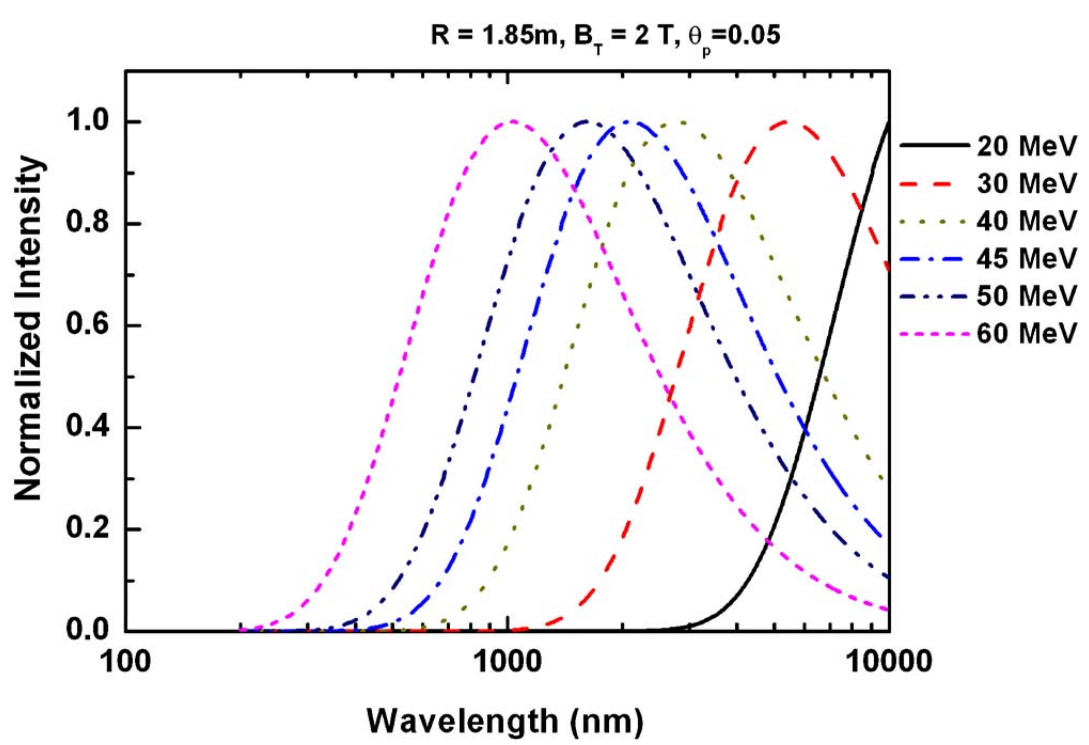
\includegraphics[width=14cm]{image46.png}
\caption{\label{fig:synchrotron3}不同逃逸电子能量的同步辐射谱\cite{RN1879}($R0=1.85$,$B_T=2T$,$v_⊥/v_∥ =0.05$)}
\end{figure}

\begin{figure}[ht]
\centering
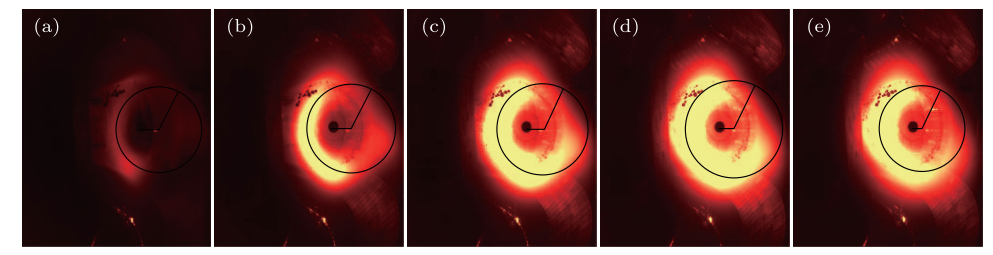
\includegraphics[width=14cm]{image47.png}
\caption{\label{fig:synchrotron4}EAST放电不同时刻逃逸电子同步辐射通过远红外相机成像\cite{RN1879},(a)1.46s,(b)1.52s,(c)1.58s,(d)1.64s,(e)1.70s。}
\end{figure}
\clearpage
\subsection{	电子回旋辐射诊断}
电子回旋辐射诊断主要通过测量托卡马克等离子体中不同电子回旋频率的辐射信号来分析等离子体中电子温度分布(或涨落)。从技术路线上看主要有三种实现方式,分别是一维电子回旋辐射诊断(ECE)、二维电子回旋辐射成像诊断(ECEI)以及迈克尔逊干涉仪。其中ECE和ECEI在技术路线上方法基本一致,都是通过外差降频的方式实现对辐射信号的测量,只是相对ECE,ECEI拥有大尺度光学透镜,能够对等离子体直接成像,具有实现大尺度高时间空间分辨率优势。而迈克尔逊干涉仪则利用空间傅里叶分析实现对电子回旋辐射宽谱范围测量,频谱覆盖范围可从几十Ghz到几百Ghz,但时间分辨率只有ms量级\cite{RN743}。以ECEI系统为例,传统上用于ECEI诊断的电子回旋辐射需要满足3个条件:其一,电子回旋辐射需要保证能从等离子体中传出来,不能被反射和吸收;其二,电子回旋辐射需要满足光学厚条件,这样才能保证辐射强度和共振层温度正比关系,即黑体辐射条件;其三,电子辐射频率和托卡马克大半径位置要满足一一对应关系,也就意味着在观测区间内,电子回旋频率不能和其它谐波频率有重叠,一般情况下我们用二次X模可以满足这些条件。对于非热化电子,通常其产生条件是低密度等离子体环境,一般不满足光学厚条件。另一方面,在非热平衡条件下由于电子回旋辐射和$β_⊥$具有非线性关系,辐射变化强烈依赖于$β_⊥$值(\autoref{fig:etamax}),此时超热电子的回旋辐射强度远大于背景热电子的回旋辐射强度,电子回旋辐射信号的分析就需要结合计算机模拟和其它诊断完成。通过结合低时间分辨宽频测量的迈克尔逊干涉仪和大尺度高时间空间分辨的电子回旋辐射诊断可以互相弥补不足,获得更多有效信息。在D.J. Campbell\cite{RN726}的工作里有两者结合的经典实验研究,简要介绍如下:
\begin{figure}[ht]
\centering
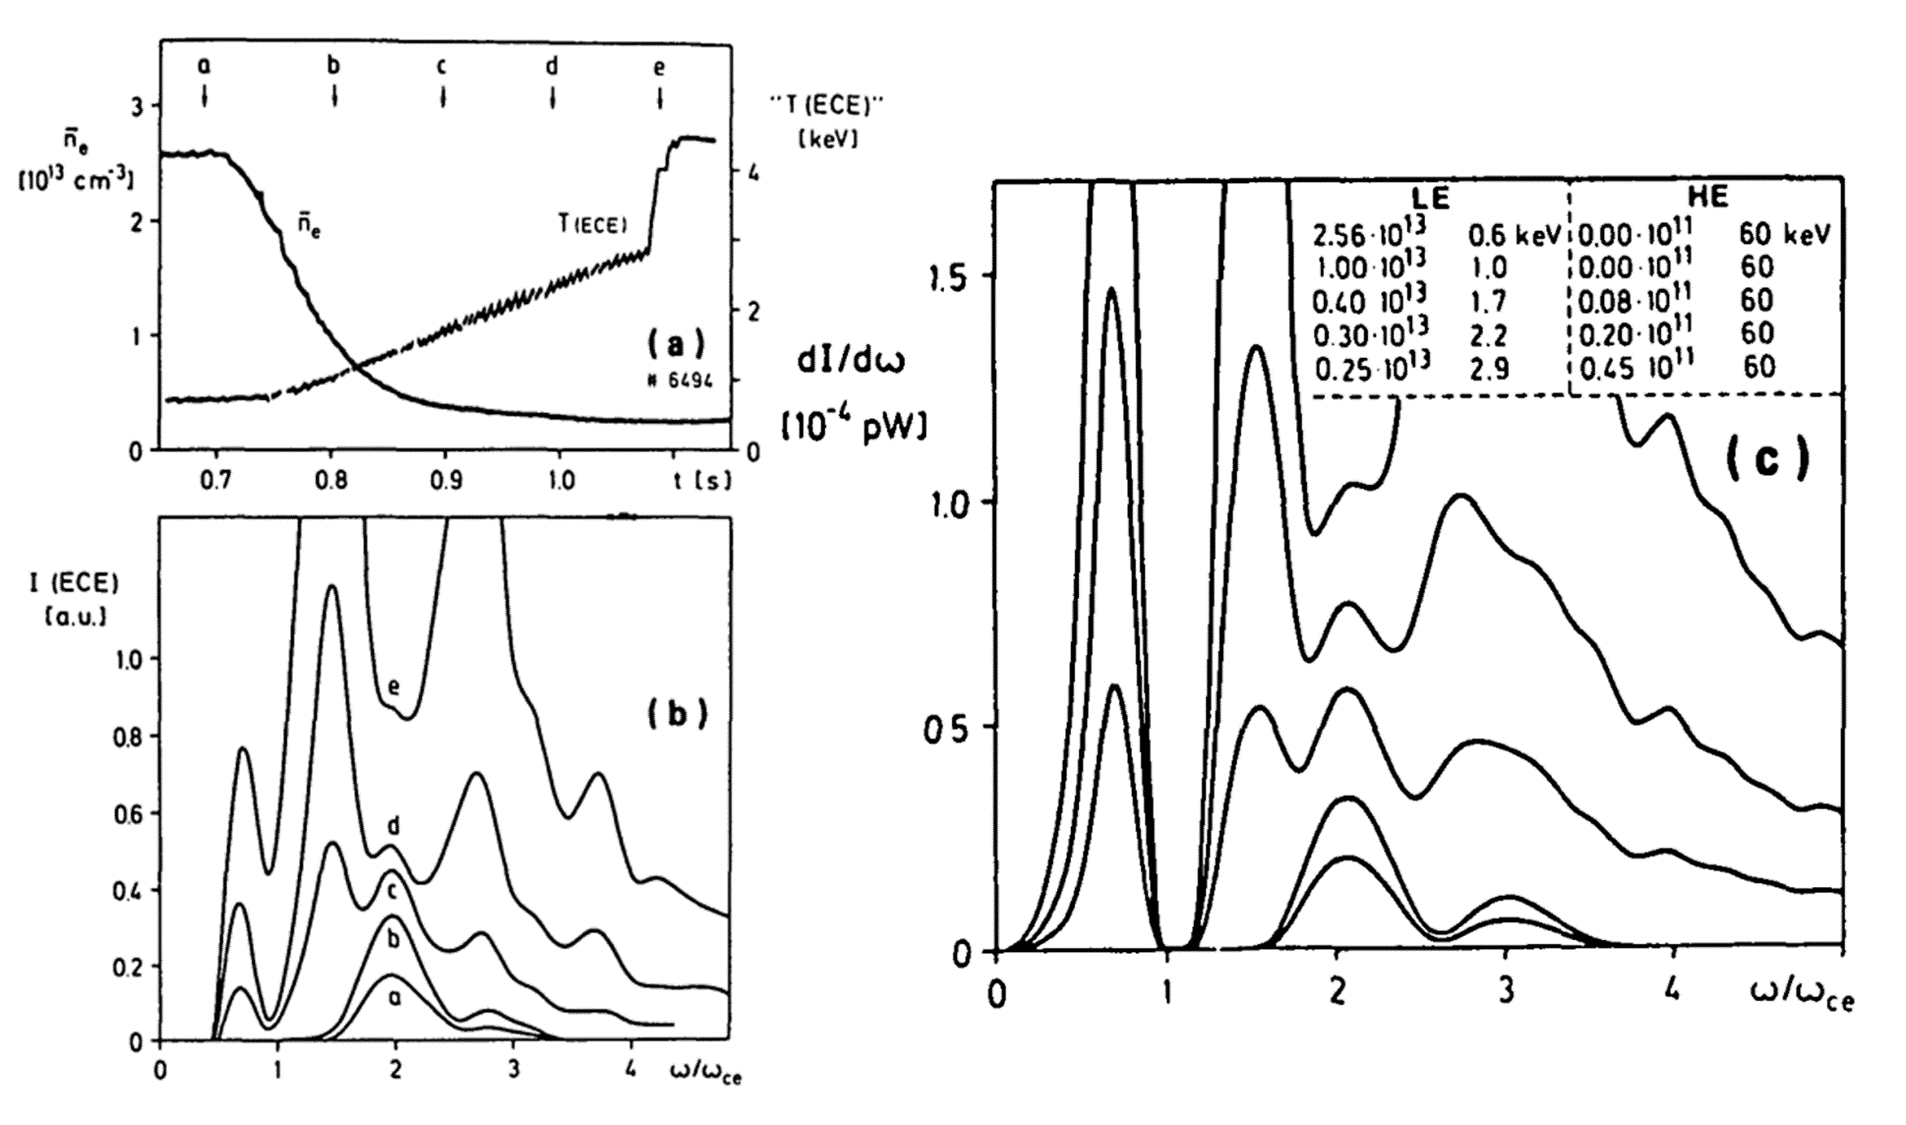
\includegraphics[width=15cm]{image48_1.png}
\caption{\label{fig:ECEspec}从热等离子体到非热等离子体演化过程中电子回旋辐射特征图\cite{RN726}。(a) 线平均等离子体密度$n_e$和表示为等效温度的2$ω_{ce} (0)-X$模电子回旋辐射强度。(b)标签a-e时刻测量得到的电子回旋辐射谱分布。(c)利用双能分布模拟得到辐射谱分布,其中包括低能部分(LE)和高能部分(HE),低能部分为热分布,高能部分为超热分布,通过改变分布函数密度和能量拟合辐射谱形状}
\end{figure}

在低密度放电条件下(通常指$ω_{pe}/ω_{ce} <1$,其中$ω_{pe}$表示电子等离
子频率,$ω_{ce}$表示电子回旋频率),由于电子之间碰撞频率降低,电子在电
场驱动下易形成偏离热分布的非热化电子。如果对分布函数采用一定的简化形
式,使得辐射谱形状能够通过有限的分布参数拟合获得,这样根据辐射谱的形状研究非热化电子就具备一定的可行性。其中一个分布函数简化方法就是双能分
布,将分布函数分为高能部分和低能部分,低能部分对应主体等离子体的密度和温度,用麦氏分布描述。高能部分主要对应偏离主体分布的非热化电子。通过对高能
部分采用不同分布函数形式计算发现:当垂直方向平均能量超过30keV后,对于不同的高能电子分布形式,只要密度和垂直方向平均能量相同,辐射谱的形状就没有明显差别。D.J. Campbell\cite{RN726}对这种现象的解释是高于$3ω_{ce}$辐射频率部分由于
各谐波分量之间相互重叠导致结构平滑,不能反映分布函数的细节。在平均能量
相同的前提下,谱的形状对分布函数并不敏感。因此高能部分可以采用相对论麦
氏分布模型表示,这样就可以根据高能部分和低能部分的密度和平均能量唯一的拟合出辐射谱结构。
\par 根据这个方法,1984年D.J. Campbell分别利用快速迈克尔逊干涉仪和多色仪测量了ASDEX托卡马克装置上非热化电子辐射[139]。迈克尔逊干涉仪通过15ms空间傅里叶变换得到$ω_{ce} (0)-5ω_{ce} (0)$区间的电子回旋辐射谱(这里$ω_{ce} (0)$表示磁轴位置处电子回旋频率),而多色仪利用光栅可以实现单频率高时间分辨测量,这两种诊断的视角均在托卡马克中平面沿着径向方向。除此之外,还有汤姆逊散射系统用于监测等离子体热电子密度和热电子温度。为了获得低密度放电条件,通常在正常的放电下($B_T (0)=2.2T$,$I_p=250-350kA$,$n_e=(2-3)×10^{13} cm^{-3}$,$T_e=600-700eV)$通过控制注入$D_2$气体,将等离子体密度降低到设定的值(通常是$(2-3)×10^{12} cm^{-3}$)。如\autoref{fig:ECEspec}所示,当在0.7s关闭气体注入时,随着等离子体密度下降至低密度平台区间,等离子体芯部ECE信号稳定上升然后在1.07s时突然升高并导致信号饱和。a-e时刻对应电子回旋辐射谱如\autoref{fig:ECEspec}(b)所示。根据双能分布模型,其中低能电子密度和能量由实验测量获得,通过拟合即可得到a-e过程中高能部分电子密度和垂直方向平均能量,如\autoref{fig:ECEspec}(c)。关于在1.07s处为什么会突然上升,Campbell没有详细的展开研究,只是猜测可能是反常多普勒效应导致速度出现散射,本文在\autoref{sec:exp_ece}也对类似的这种现象展开讨论,并得到了与之不同的结论。\par
D.J. Campbell 的方虽然可以实现对非热化电子数量和能量的拟合,但是由于其诊断视角在中平面沿着半径方向,纵场的变化也一定会对谱分布结构带来影响,因此1990年G.Taylor采用垂直方向接收电子回旋辐射谱\cite{RN2037}。如\autoref{fig:VECE}所示,该诊断可以通过调节反射镜实现三个不同径向位置垂直方向电子回旋辐射测量,由于垂直方向纵场几乎不变,因此可以获得固定纵场条件下的电子回旋辐射谱,然后使用双温分布拟合电子回旋辐射谱获得非热化电子的平均能量和数量。通过垂直方向测量电子回旋谱分布的另一个直观的优点是可以根据辐射频率估算高能电子能量,这是因为当地电子回旋频率会由于相对论效应出现展宽,通过测量不同能量对应辐射频率的强度原则上就能研究非热化电子能量分布。但是实际上由于壁面反射导致测量信号并不一定来自对应测量径向位置通道的信号,实验中还是有很多需要考虑的问题,例如评估壁反射对信号的污染,如何抑制壁反射等。 M. Farník在研究COMPASS托卡马克上逃逸电子回旋辐射时对此有过详细的分析\cite{RN823}。
\begin{figure}[ht]
\centering
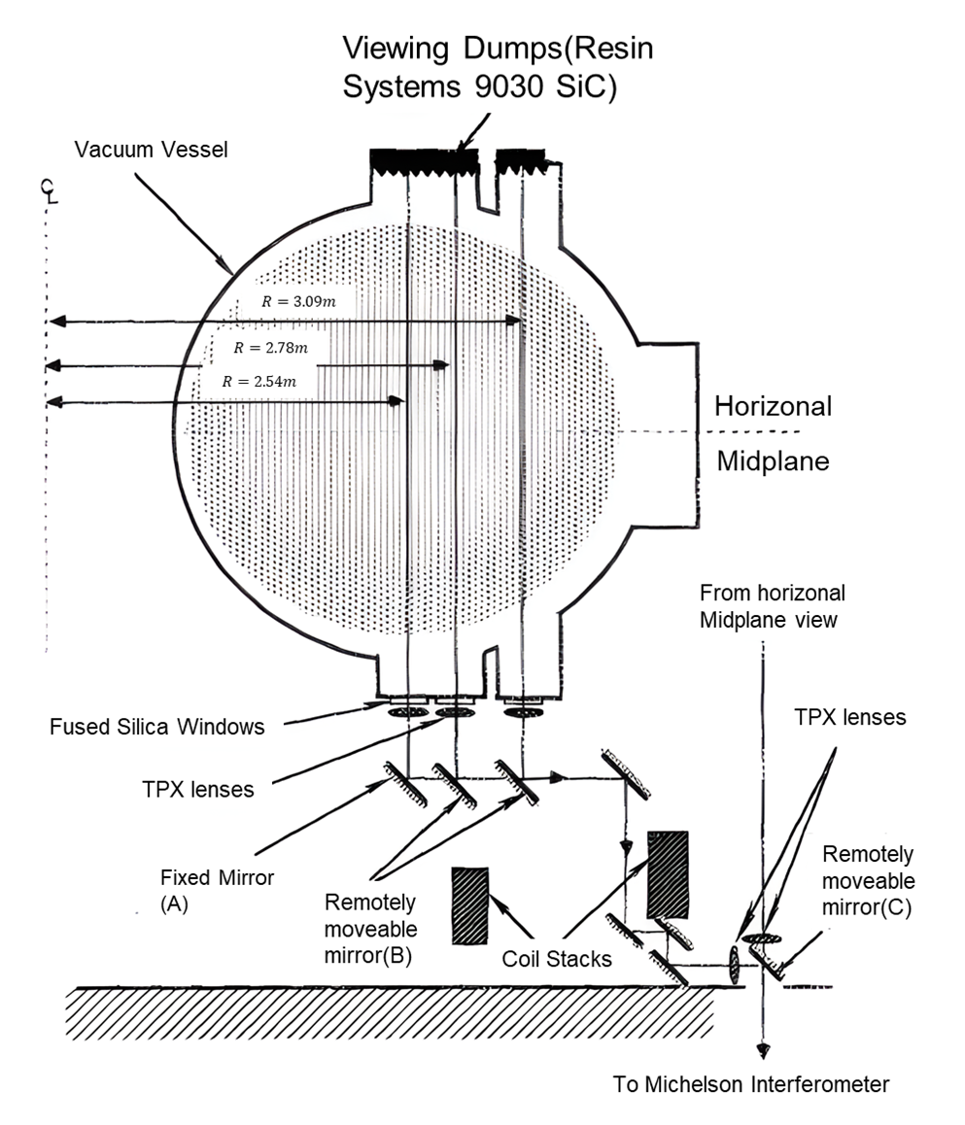
\includegraphics[width=12cm]{image49_1.png}
\caption{\label{fig:VECE}TFTR垂直方向电子回旋辐射诊断\cite{RN2037}}
\end{figure}
  \par 尽管双能分布简化了分布函数的复杂度,但不免会丢失很多细节上的信息。如果能建立分布函数演化模型,计算不同时刻下分布函数形状和电子回旋谱信号,同时结合实验过程中用到的电子回旋辐射诊断,对比模拟辐射信号和实验中观测到的辐射信号,这将会对非热化电子辐射以及其背后的物理过程有更加直观的理解。为了实现这个目的,在接下来的章节中本文将依次介绍不同速度分布下电子回旋辐射信号的计算以及电子速度分布演化的数值模拟方法,为实验测量所得辐射结构提供数值研究平台。
\section{小结}
本章给出了等离子体中电子速度分布函数的动理学模型以及探测非热化电子的
相关诊断方法。在非热化电子的动理学模型中,本章讨论了小角度散射的Fokker-Planck碰撞算符$C[f]$、雪崩算符$S_A[f]$、辐射阻尼算符$\frac{\partial}{\partial \boldsymbol{p}} \cdot\left(F_{\mathrm{rad}} f\right)$、电场驱动算符以及准线性扩散算符$D[f]$等。非热电子理论将用于动理学计算程序中,以实现非热电子演化的数值模拟。关于非热电子诊断方面主要介绍了同步辐射诊断,轫致辐射诊断以及电子回旋辐射诊断。为了将电子速度分布演化过程与实验诊断数据相互比较,在下一章中我们主要研究电子回旋辐射诊断的数值模拟平台,解决任意电子速度分布映射到电子回旋辐射的正向过程,进而实现与实验现象中电子回旋辐射信号的直接对比,这样我们的模拟数据就有了实验参考,而不是脱轨的数值幻象。 

















